\clearpage

\appendix

\section{Idiosyncratic returns for VC funds}
\label{sec:vc_errors}



% Factor Model Returns + Errors for VC

\begin{figure}[H]
	\centering
	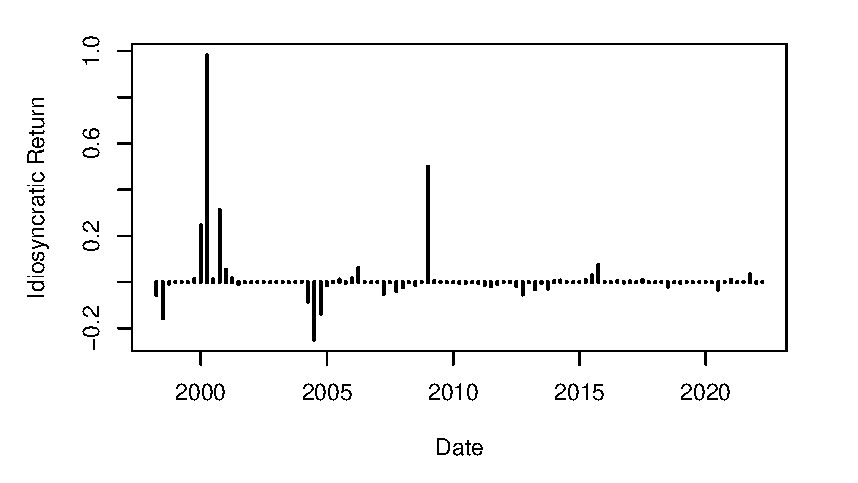
\includegraphics{Figures/XErrorSeriesVC}
	\caption{Idiosyncratic returns estimated by componentwise $L_2$ boosting for fund type VC in the period from 1998-03-31 until 2022-03-31.}
	\label{fig:clb_idio_vc}
\end{figure}

\begin{figure}[H]
	\centering
	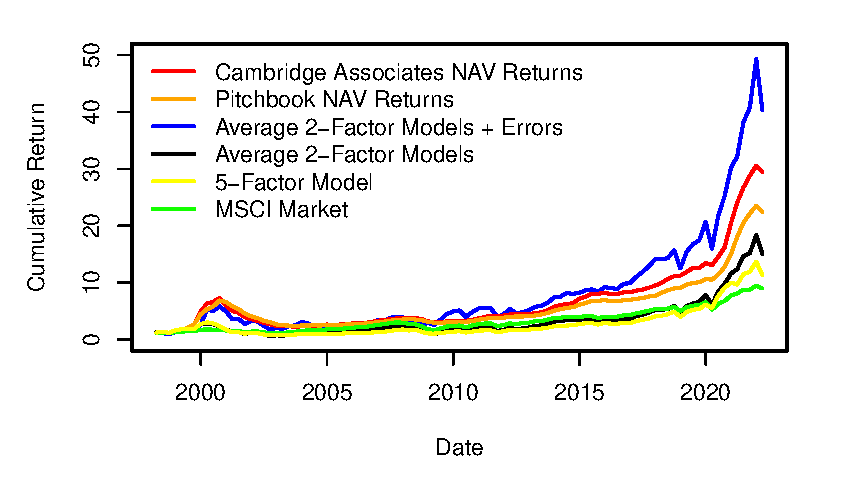
\includegraphics{Figures/XTotalErrorSeriesVC}
	\caption{
		Comparison between the total returns for fund type VC implied by our two-factor ensemble and our two-factor ensemble plus the error term from Figure \ref{fig:clb_idio}.
		Both series are contrasted against the NAV Return indices provided by Cambridge Associates and Pitchbook and the MSCI stock market index in the period 1998-03-31 until 2022-03-31.
	}
	\label{fig:clb_total_vc}
\end{figure}

\begin{figure}[H]
	\centering
	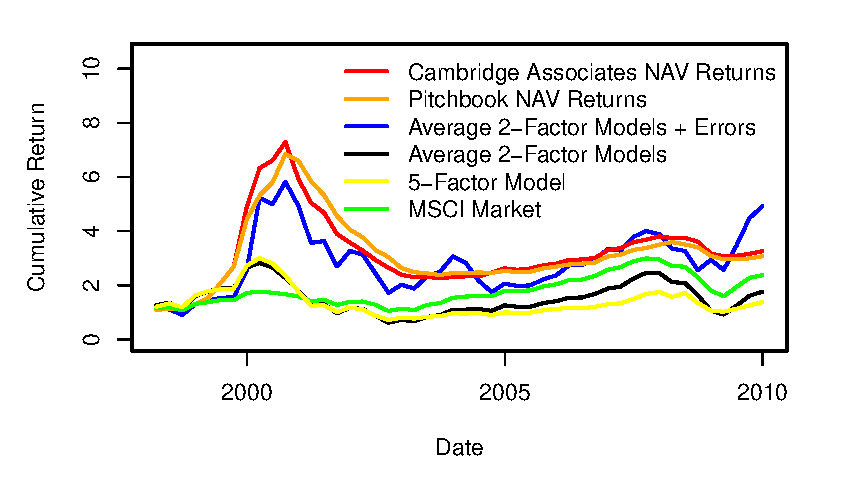
\includegraphics{Figures/XTotalErrorSeriesVCpre2010}
	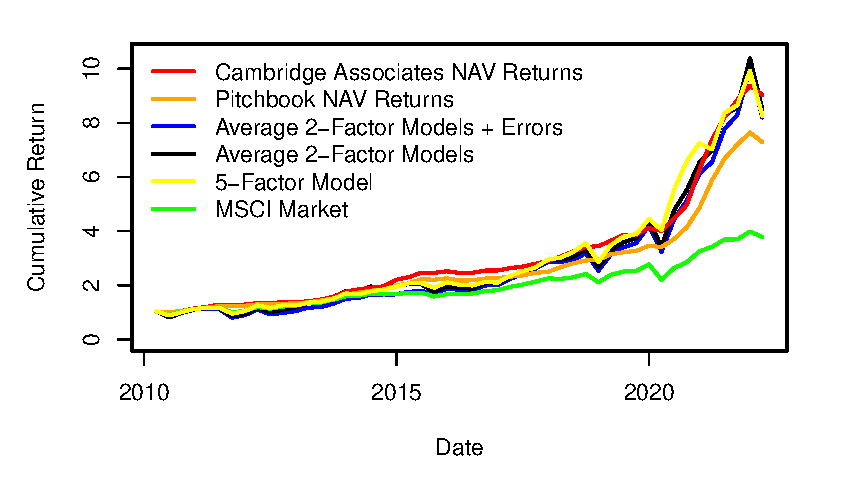
\includegraphics{Figures/XTotalErrorSeriesVCpost2010}
	\caption{
		In these two subplots, we split the full time series from Figure \ref{fig:clb_total_vc} into a pre-2010 and post-2010 period.
		Similar to the BO case in Figure \ref{fig:clb_pre_post_2010}, we see diverse return time series pre 2010 but after 2010 all three public factor model returns (with and without error terms) closely match the two NAV return series.
	}
	\label{fig:clb_pre_post_2010_vc}
\end{figure}



\section{Idiosyncratic returns for RE funds}
\label{sec:re_errors}



% Factor Model Returns + Errors for RE

\begin{figure}[H]
	\centering
	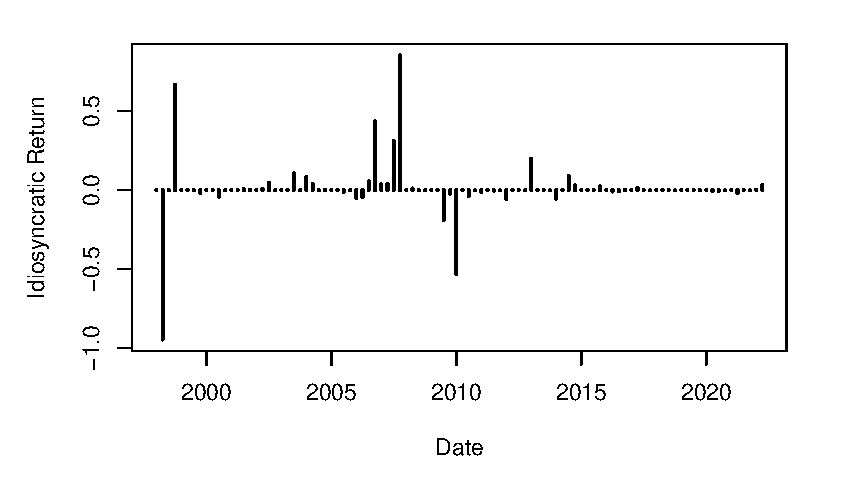
\includegraphics{Figures/XErrorSeriesRE}
	\caption{Idiosyncratic returns estimated by componentwise $L_2$ boosting for fund type RE in the period from 1998-03-31 until 2022-03-31.}
	\label{fig:clb_idio_re}
\end{figure}

\begin{figure}[H]
	\centering
	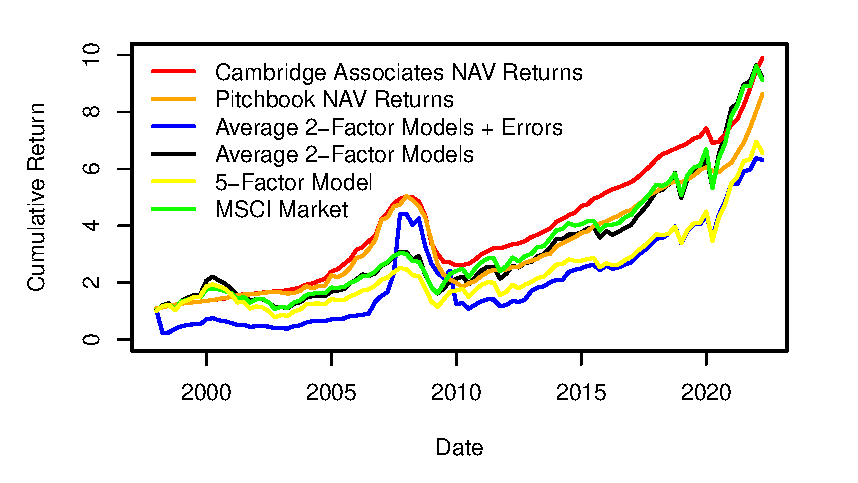
\includegraphics{Figures/XTotalErrorSeriesRE}
	\caption{
		Comparison between the total returns for fund type RE implied by our two-factor ensemble and our two-factor ensemble plus the error term from Figure \ref{fig:clb_idio_re}.
		Both series are contrasted against the NAV Return indices provided by Cambridge Associates and Pitchbook and the MSCI stock market index in the period 1998-03-31 until 2022-03-31.
	}
	\label{fig:clb_total_re}
\end{figure}

\begin{figure}[H]
	\centering
	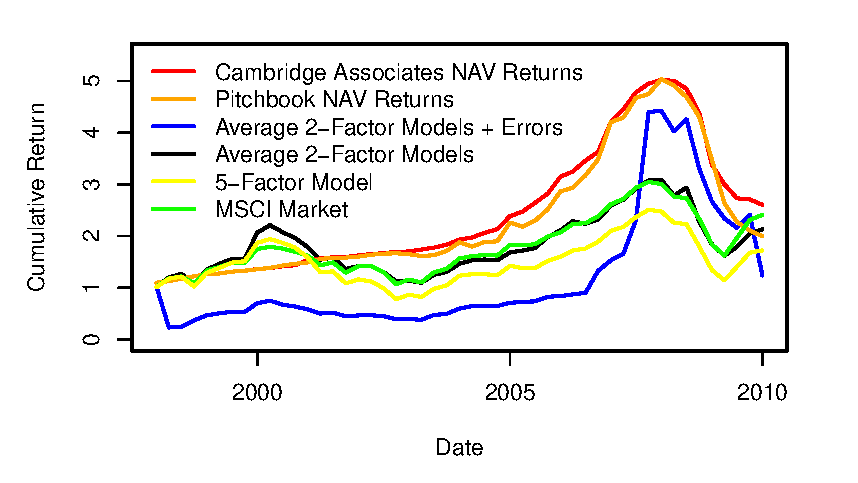
\includegraphics{Figures/XTotalErrorSeriesREpre2010}
	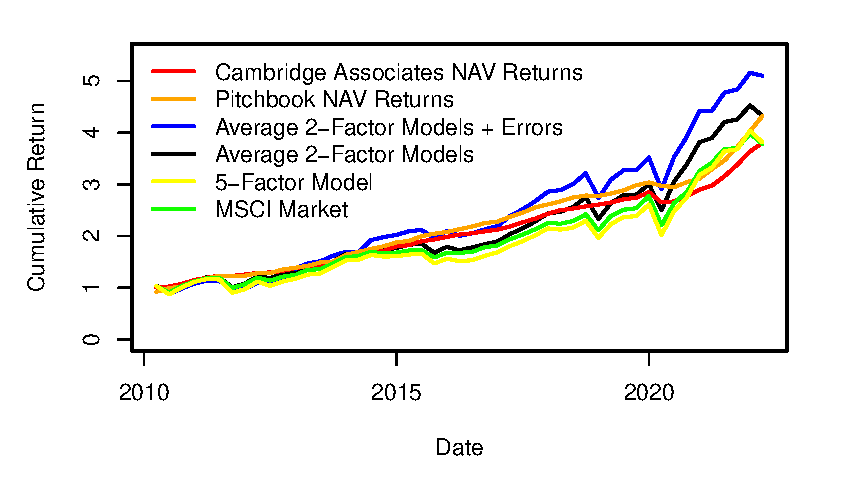
\includegraphics{Figures/XTotalErrorSeriesREpost2010}
	\caption{
		In these two subplots, we split the full time series from Figure \ref{fig:clb_total_re} into a pre-2010 and post-2010 period.
		Again, similar to the BO and VC cases in Figure \ref{fig:clb_pre_post_2010} and  Figure \ref{fig:clb_pre_post_2010_vc}, we see diverse return time series pre 2010 but after 2010 all three public factor model returns (with and without error terms) closely match the two NAV return series.
	}
	\label{fig:clb_pre_post_2010_RE}
\end{figure}


\section{Idiosyncratic returns for DD funds}
\label{sec:dd_errors}

% Factor Model Returns + Errors for DD

\begin{figure}[H]
	\centering
	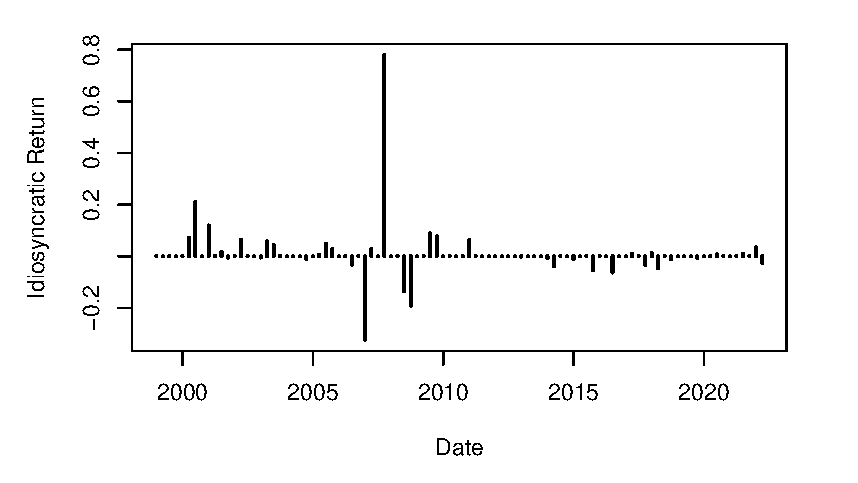
\includegraphics{Figures/XErrorSeriesDD}
	\caption{Idiosyncratic returns estimated by componentwise $L_2$ boosting for fund type DD in the period from 1998-03-31 until 2022-03-31.}
	\label{fig:clb_idio_DD}
\end{figure}

\begin{figure}[H]
	\centering
	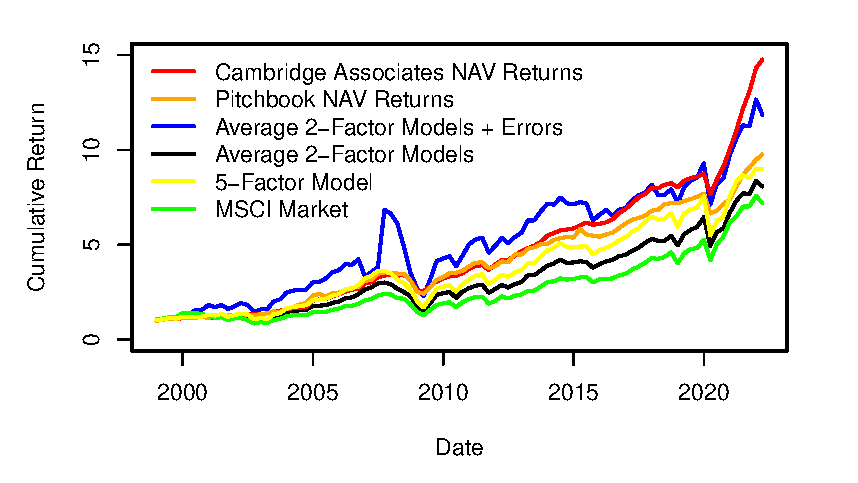
\includegraphics{Figures/XTotalErrorSeriesDD}
	\caption{
		Comparison between the total returns for fund type RE implied by our two-factor ensemble and our two-factor ensemble plus the error term from Figure \ref{fig:clb_idio_DD}.
		Both series are contrasted against the NAV Return indices provided by Cambridge Associates and Pitchbook and the MSCI stock market index in the period 1998-03-31 until 2022-03-31.
	}
	\label{fig:clb_total_DD}
\end{figure}

\begin{figure}[H]
	\centering
	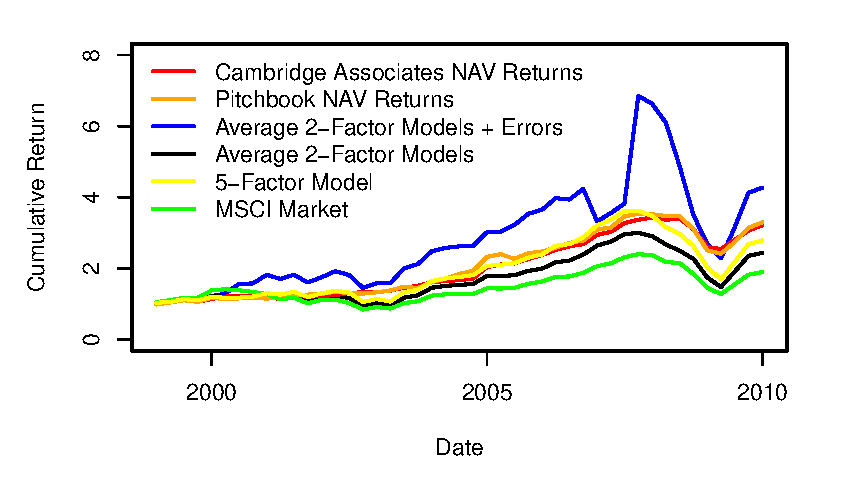
\includegraphics{Figures/XTotalErrorSeriesDDpre2010}
	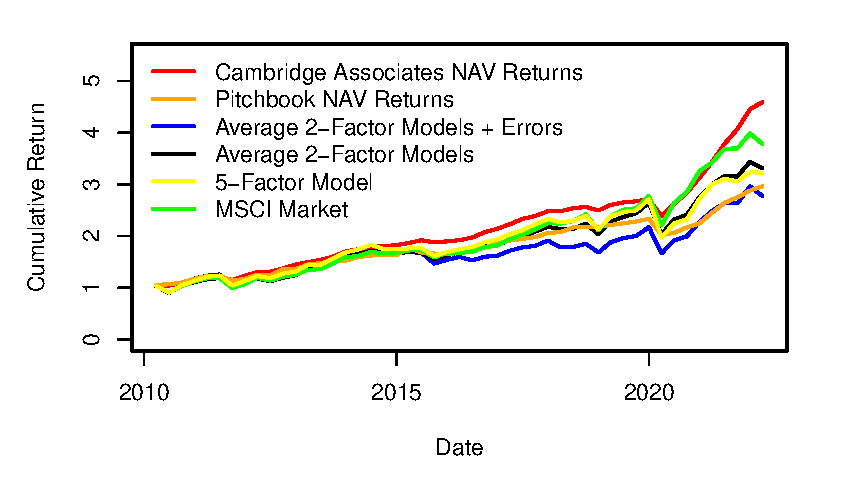
\includegraphics{Figures/XTotalErrorSeriesDDpost2010}
	\caption{
		In these two subplots, we split the full time series from Figure \ref{fig:clb_total_DD} into a pre-2010 and post-2010 period.
		Again, similar to the BO and VC cases in Figure \ref{fig:clb_pre_post_2010} and  Figure \ref{fig:clb_pre_post_2010_vc}, we see diverse return time series pre 2010 but after 2010 all three public factor model returns (with and without error terms) closely match the two NAV return series.
	}
	\label{fig:clb_pre_post_2010_DD}
\end{figure}


\section{Idiosyncratic returns for INF funds}
\label{sec:inf_errors}

% Factor Model Returns + Errors for INF

\begin{figure}[H]
	\centering
	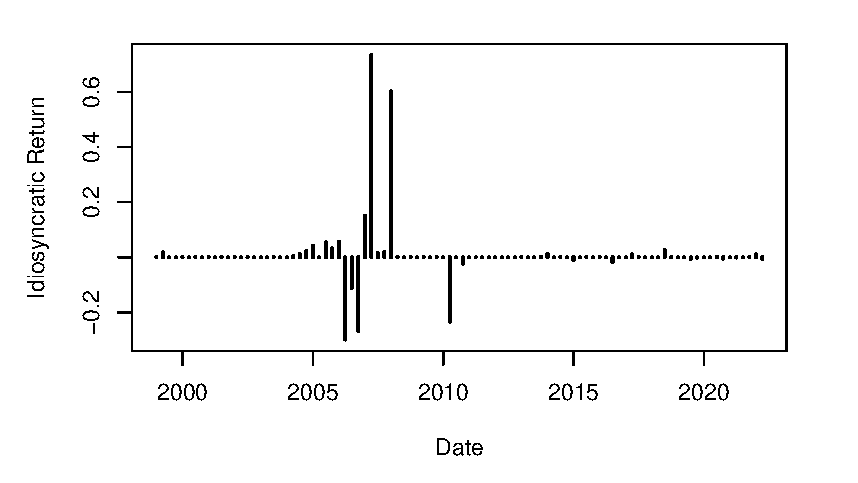
\includegraphics{Figures/XErrorSeriesINF}
	\caption{Idiosyncratic returns estimated by componentwise $L_2$ boosting for fund type DD in the period from 1998-03-31 until 2022-03-31.}
	\label{fig:clb_idio_inf}
\end{figure}

\begin{figure}[H]
	\centering
	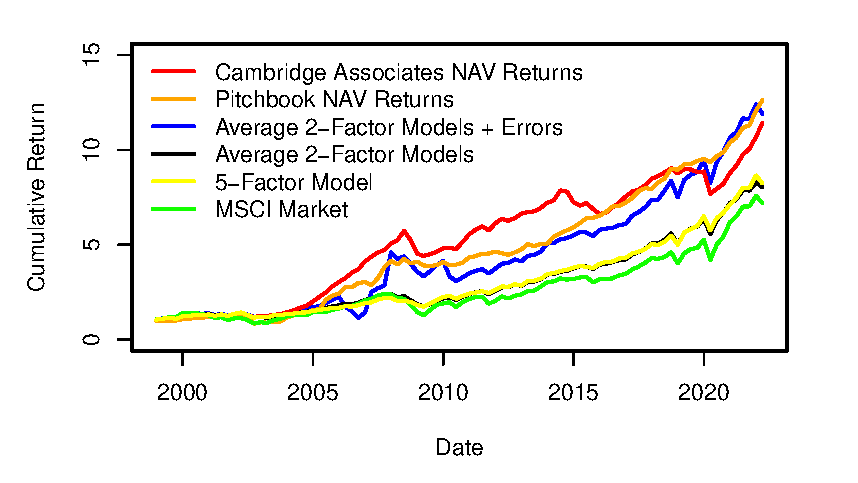
\includegraphics{Figures/XTotalErrorSeriesINF}
	\caption{
		Comparison between the total returns for fund type RE implied by our two-factor ensemble and our two-factor ensemble plus the error term from Figure \ref{fig:clb_idio_inf}.
		Both series are contrasted against the NAV Return indices provided by Cambridge Associates and Pitchbook and the MSCI stock market index in the period 1998-03-31 until 2022-03-31.
	}
	\label{fig:clb_total_inf}
\end{figure}

\begin{figure}[H]
	\centering
	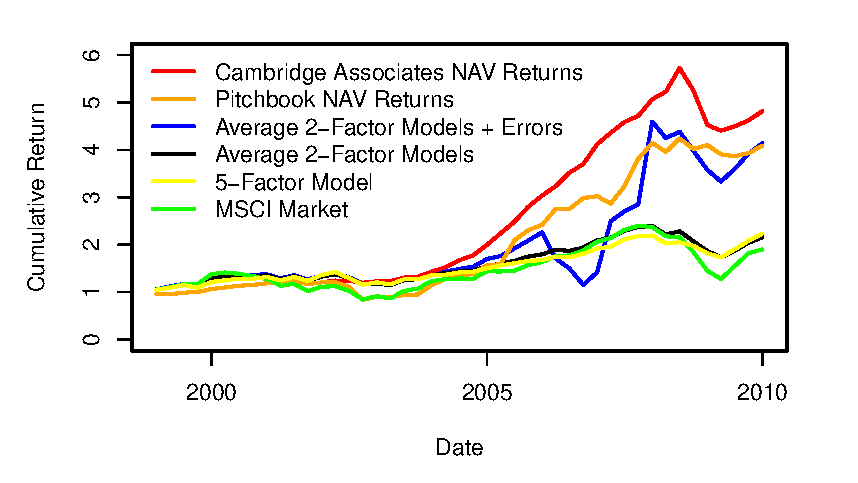
\includegraphics{Figures/XTotalErrorSeriesINFpre2010}
	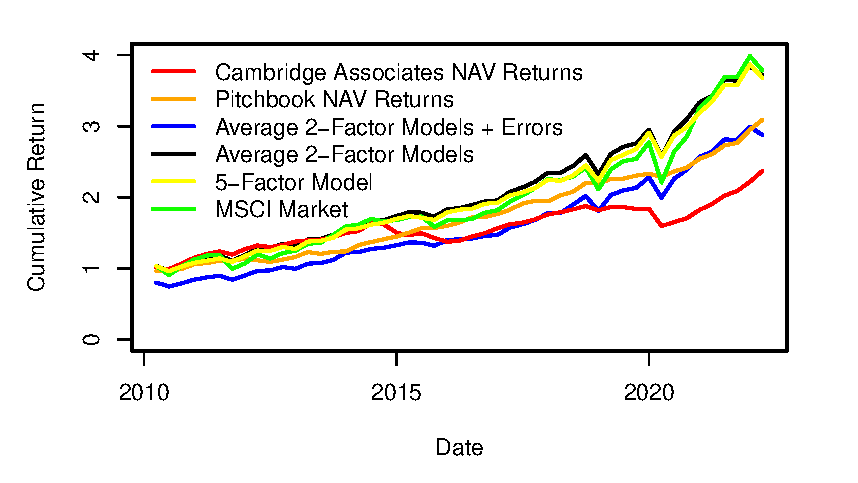
\includegraphics{Figures/XTotalErrorSeriesINFpost2010}
	\caption{
		In these two subplots, we split the full time series from Figure \ref{fig:clb_total_inf} into a pre-2010 and post-2010 period.
		Again, similar to the BO and VC cases in Figure \ref{fig:clb_pre_post_2010} and  Figure \ref{fig:clb_pre_post_2010_vc}, we see diverse return time series pre 2010 but after 2010 all three public factor model returns (with and without error terms) closely match the two NAV return series.
	}
	\label{fig:clb_pre_post_2010_inf}
\end{figure}


\section{Idiosyncratic returns for NATRES funds}
\label{sec:natres_errors}

% Factor Model Returns + Errors for NATRES

\begin{figure}[H]
	\centering
	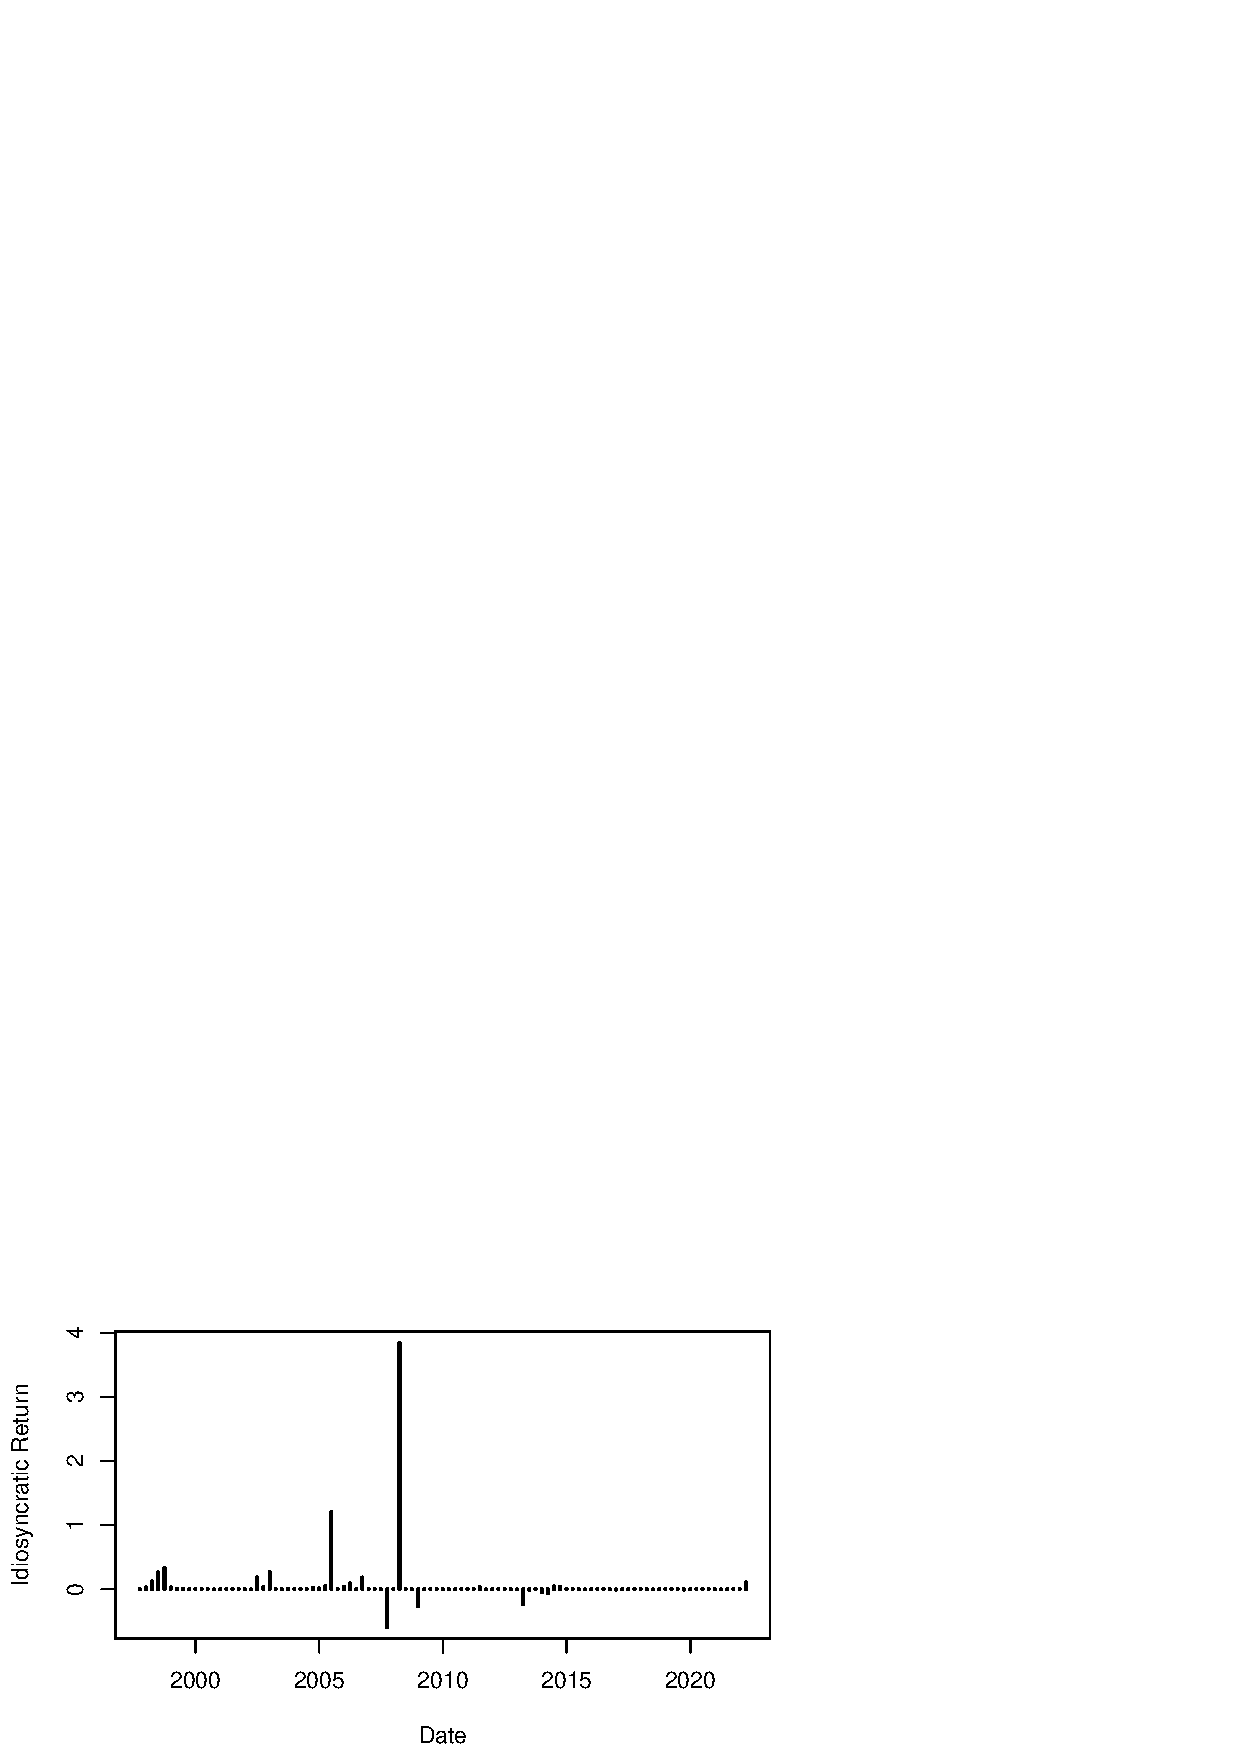
\includegraphics{Figures/XErrorSeriesNATRES}
	\caption{Idiosyncratic returns estimated by componentwise $L_2$ boosting for fund type DD in the period from 1998-03-31 until 2022-03-31.}
	\label{fig:clb_idio_natres}
\end{figure}

\begin{figure}[H]
	\centering
	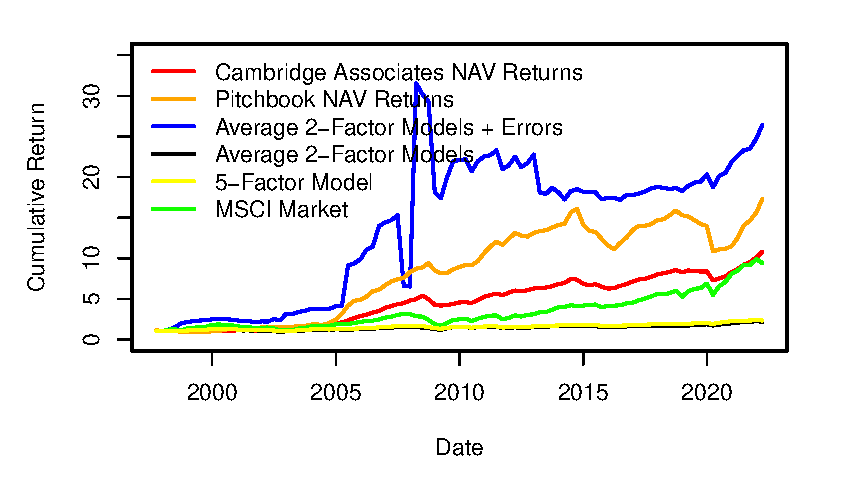
\includegraphics{Figures/XTotalErrorSeriesNATRES}
	\caption{
		Comparison between the total returns for fund type RE implied by our two-factor ensemble and our two-factor ensemble plus the error term from Figure \ref{fig:clb_idio_natres}.
		Both series are contrasted against the NAV Return indices provided by Cambridge Associates and Pitchbook and the MSCI stock market index in the period 1998-03-31 until 2022-03-31.
	}
	\label{fig:clb_total_natres}
\end{figure}

\begin{figure}[H]
	\centering
	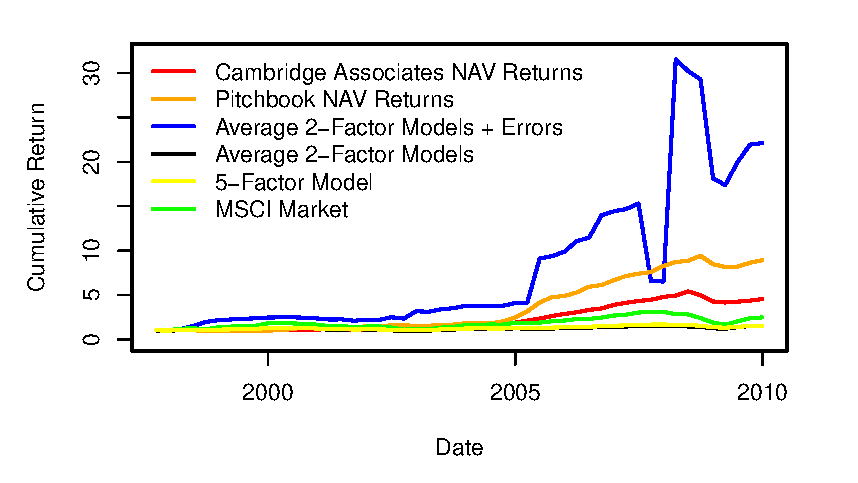
\includegraphics{Figures/XTotalErrorSeriesNATRESpre2010}
	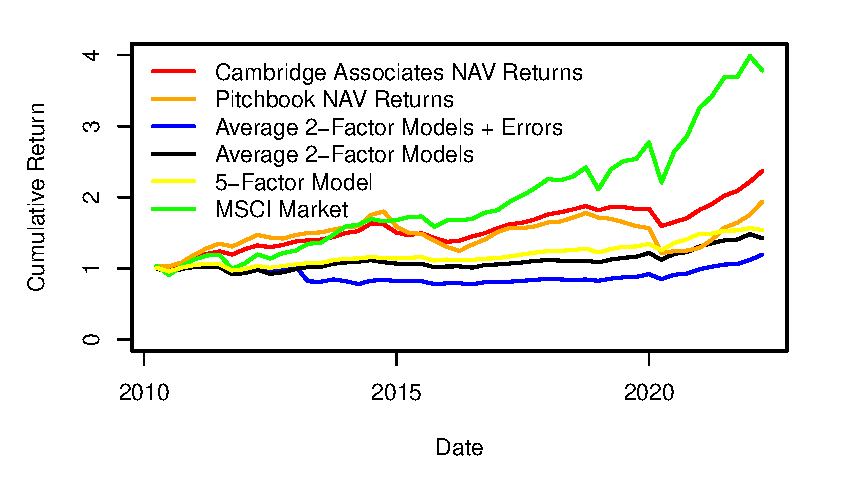
\includegraphics{Figures/XTotalErrorSeriesNATRESpost2010}
	\caption{
		In these two subplots, we split the full time series from Figure \ref{fig:clb_total_natres} into a pre-2010 and post-2010 period.
	}
	\label{fig:clb_pre_post_2010_natres}
\end{figure}


\section{Idiosyncratic returns for MEZZ funds}
\label{sec:MEZZ_errors}

% Factor Model Returns + Errors for MEZZ

\begin{figure}[H]
	\centering
	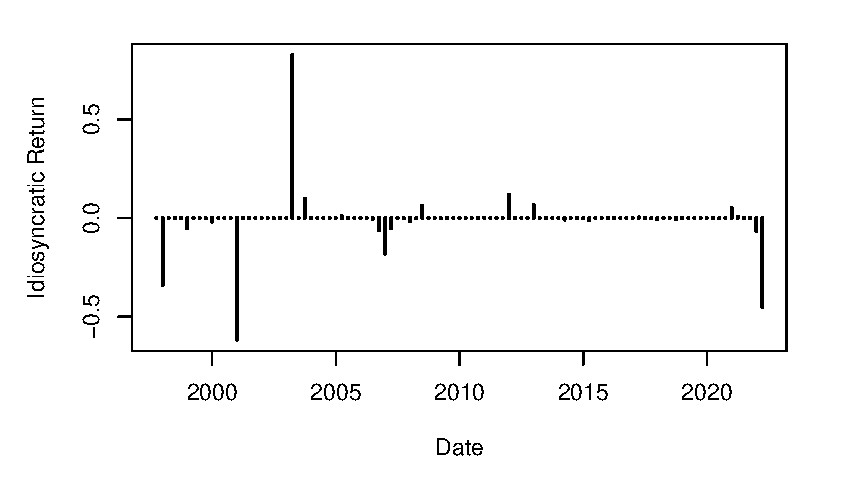
\includegraphics{Figures/XErrorSeriesMEZZ}
	\caption{Idiosyncratic returns estimated by componentwise $L_2$ boosting for fund type DD in the period from 1998-03-31 until 2022-03-31.}
	\label{fig:clb_idio_MEZZ}
\end{figure}

\begin{figure}[H]
	\centering
	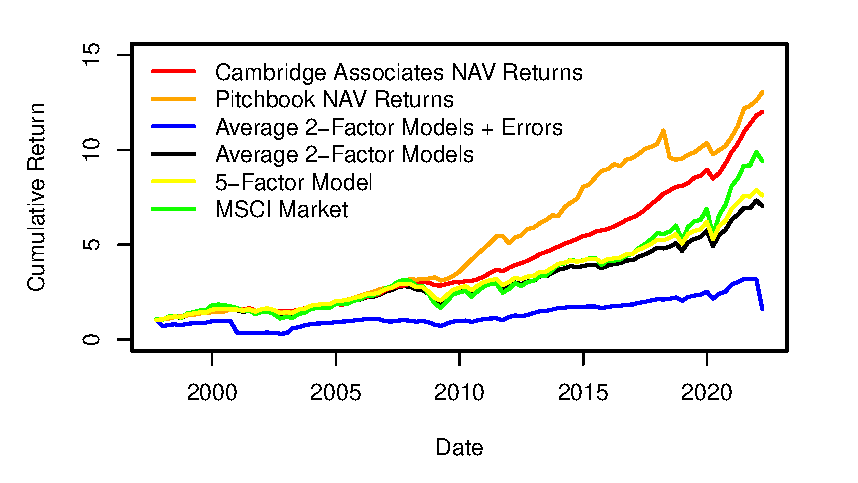
\includegraphics{Figures/XTotalErrorSeriesMEZZ}
	\caption{
		Comparison between the total returns for fund type RE implied by our two-factor ensemble and our two-factor ensemble plus the error term from Figure \ref{fig:clb_idio_MEZZ}.
		Both series are contrasted against the NAV Return indices provided by Cambridge Associates and Pitchbook and the MSCI stock market index in the period 1998-03-31 until 2022-03-31.
	}
	\label{fig:clb_total_MEZZ}
\end{figure}

\begin{figure}[H]
	\centering
	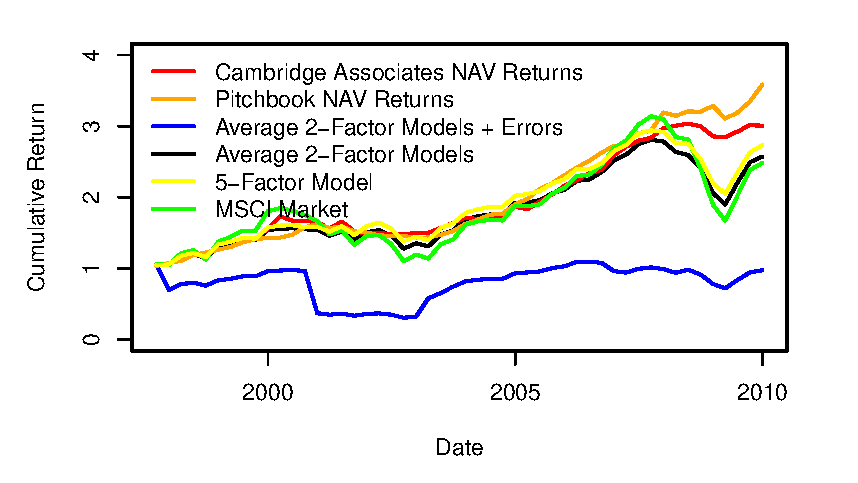
\includegraphics{Figures/XTotalErrorSeriesMEZZpre2010}
	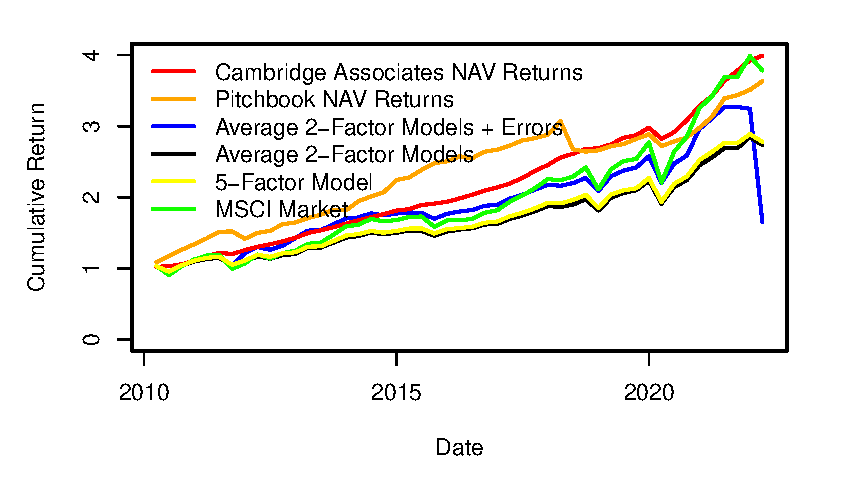
\includegraphics{Figures/XTotalErrorSeriesMEZZpost2010}
	\caption{
		In these two subplots, we split the full time series from Figure \ref{fig:clb_total_MEZZ} into a pre-2010 and post-2010 period.
	}
	\label{fig:clb_pre_post_2010_MEZZ}
\end{figure}


\section{Idiosyncratic returns for PD funds}
\label{sec:PD_errors}

% Factor Model Returns + Errors for PD

\begin{figure}[H]
	\centering
	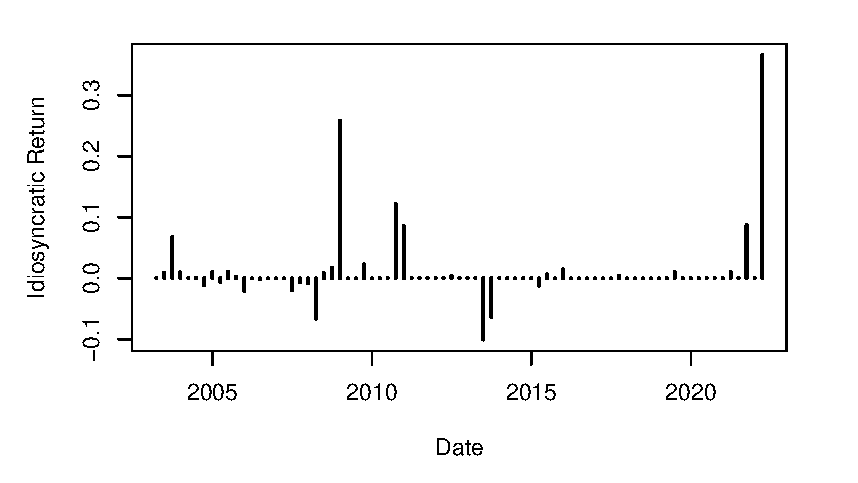
\includegraphics{Figures/XErrorSeriesPD}
	\caption{Idiosyncratic returns estimated by componentwise $L_2$ boosting for fund type DD in the period from 1998-03-31 until 2022-03-31.}
	\label{fig:clb_idio_PD}
\end{figure}

\begin{figure}[H]
	\centering
	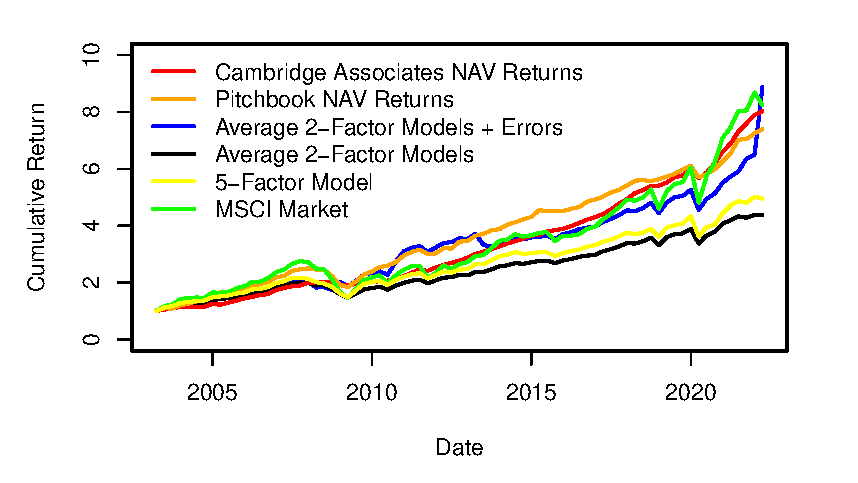
\includegraphics{Figures/XTotalErrorSeriesPD}
	\caption{
		Comparison between the total returns for fund type RE implied by our two-factor ensemble and our two-factor ensemble plus the error term from Figure \ref{fig:clb_idio_PD}.
		Both series are contrasted against the NAV Return indices provided by Cambridge Associates and Pitchbook and the MSCI stock market index in the period 1998-03-31 until 2022-03-31.
	}
	\label{fig:clb_total_PD}
\end{figure}

\begin{figure}[H]
	\centering
	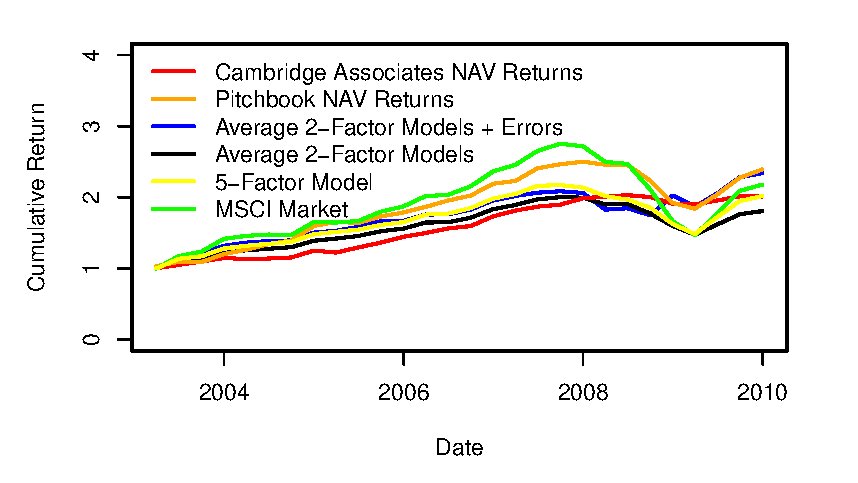
\includegraphics{Figures/XTotalErrorSeriesPDpre2010}
	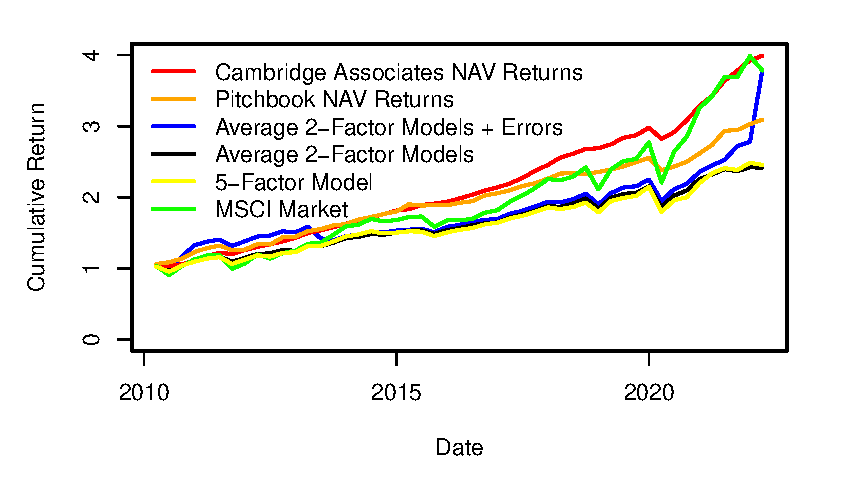
\includegraphics{Figures/XTotalErrorSeriesPDpost2010}
	\caption{
		In these two subplots, we split the full time series from Figure \ref{fig:clb_total_PD} into a pre-2010 and post-2010 period.
	}
	\label{fig:clb_pre_post_2010_PD}
\end{figure}